\documentclass[11pt,oneside,fontset=none]{ctexbook}

\IfFontExistsTF{Songti SC}{%
  \setCJKmainfont{Songti SC}%
  \setCJKmonofont{Songti SC}%
}{%
  \IfFontExistsTF{Noto Serif CJK SC}{%
    \setCJKmainfont{Noto Serif CJK SC}%
    \setCJKmonofont{Noto Serif CJK SC}%
  }{%
    \setCJKmainfont{FandolSong}%
    \setCJKmonofont{FandolFang}%
  }%
}
\IfFontExistsTF{Heiti SC}{%
  \setCJKsansfont{Heiti SC}%
}{%
  \IfFontExistsTF{Noto Sans CJK SC}{%
    \setCJKsansfont{Noto Sans CJK SC}%
  }{%
    \setCJKsansfont{FandolHei}%
  }%
}

\usepackage[a4paper,margin=2.5cm]{geometry}
\usepackage{amsmath,amssymb}
\usepackage[colorlinks=true,linkcolor=blue!65!black,urlcolor=teal!75!black,citecolor=teal!75!black]{hyperref}
\usepackage{graphicx}
\usepackage{booktabs}
\usepackage{longtable}
\usepackage{listings}
\usepackage{xcolor}
\usepackage[framemethod=TikZ]{mdframed}
\usepackage{xurl}
\usepackage{array}
\usepackage{tabularx}
\usepackage{float}
\usepackage{multicol}
\usepackage{etoc}

\definecolor{codebg}{HTML}{F7F8FA}
\definecolor{codeframe}{HTML}{D0D7DE}
\definecolor{tipbg}{HTML}{F0F6FC}
\definecolor{tipframe}{HTML}{1B4F9C}
\definecolor{warnbg}{HTML}{FFF8EC}
\definecolor{warnframe}{HTML}{C86D14}

\lstset{
  basicstyle=\ttfamily\small,
  numbers=left,
  numberstyle=\tiny\color{gray},
  breaklines=true,
  columns=fullflexible,
  showstringspaces=false,
  tabsize=2,
  xleftmargin=2.1em,
  numbersep=8pt,
}

\mdfdefinestyle{codebox}{%
  roundcorner=4pt,%
  linecolor=codeframe,%
  linewidth=0.6pt,%
  backgroundcolor=codebg,%
  innerleftmargin=0pt,%
  innerrightmargin=6pt,%
  innertopmargin=4pt,%
  innerbottommargin=4pt,%
  skipabove=6pt,%
  skipbelow=6pt,%
}
\surroundwithmdframed[style=codebox]{lstlisting}
\let\origLstInputListing\lstinputlisting
\renewcommand{\lstinputlisting}[2][]{%
  \begin{mdframed}[style=codebox]%
    \origLstInputListing[#1]{#2}%
  \end{mdframed}%
}

\newmdenv[
  roundcorner=4pt,
  linecolor=tipframe,
  linewidth=1.2pt,
  leftline=true, rightline=false, topline=false, bottomline=false,
  backgroundcolor=tipbg,
  innertopmargin=6pt, innerbottommargin=6pt,
  innerleftmargin=10pt, innerrightmargin=10pt,
  skipabove=8pt, skipbelow=8pt
]{tipbox}

\newmdenv[
  roundcorner=4pt,
  linecolor=warnframe,
  linewidth=1.2pt,
  leftline=true, rightline=false, topline=false, bottomline=false,
  backgroundcolor=warnbg,
  innertopmargin=6pt, innerbottommargin=6pt,
  innerleftmargin=10pt, innerrightmargin=10pt,
  skipabove=8pt, skipbelow=8pt
]{warnbox}

\newcommand{\code}[1]{\texttt{#1}}

\title{11 分钟学会 tsqx：竞赛几何作图完全手册}
\author{LeyuDame}
\date{\today}

\begin{document}
\frontmatter

\begin{titlepage}
  \centering
  \vspace*{1.0cm}
  \IfFileExists{figures/fig4_ninepoint.pdf}{%
    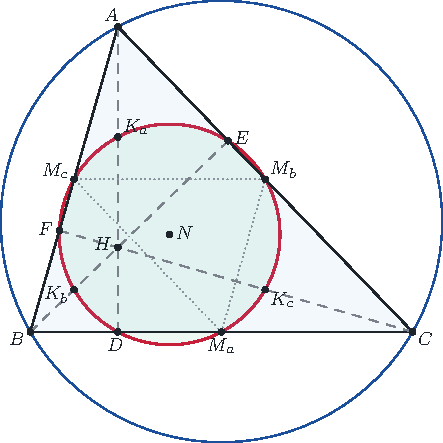
\includegraphics[width=7.5cm]{figures/fig4_ninepoint.pdf}\par
  }{%
    \fbox{\parbox{0.65\linewidth}{\centering 封面插图缺失：figures/fig4\_ninepoint.pdf}}\par
  }
  \vspace{1.2cm}
  {\Huge\bfseries 11 分钟学会 tsqx\par}
  \vspace{0.7em}
  {\Large 竞赛平面几何声明式作图、语义化配色与 AI 工作流完全手册\par}
  \vspace{1.6em}
  {\large LeyuDame\par}
  \vspace{0.4em}
  {\large \today\par}
  \vfill
  {\small\color{gray} 基于上游 \texttt{vEnhance/tsqx} 解析器源码实测编写，配套 \texttt{ldgeo.asy}、\texttt{tsqx-gen} 与 \texttt{tsqx-compiler}。\par}
\end{titlepage}

\etocsettocstyle{\begin{multicols}{2}}{\end{multicols}}
\tableofcontents
\mainmatter

% ============================================================================
\chapter{为什么在 AI 时代仍需要 TSQX}
% ============================================================================

\section{四条几何配图路线的实际边界}

准备数学竞赛讲义或试卷时，最常见的一个需求是：手头只有一段自然语言题干，需要在几分钟内配出一张数学准确、线型克制、风格与整篇讲义统一的平面几何插图。今天可以用大模型直接生成 TikZ 或 Python 绘图代码，也可以用 GeoGebra 拖拽画图。选择哪一条路线，取决于具体图形的数学结构，而不是工具的新旧。

表~\ref{tab:route-compare} 对比了四条常见路线在竞赛平面几何场景下的实际表现。

\begin{table}[htbp]
  \centering
  \caption{平面几何配图四条路线对比}
  \label{tab:route-compare}
  \small
  \begin{tabularx}{\linewidth}{@{}>{\bfseries}p{0.17\linewidth}XXXX@{}}
    \toprule
    比较维度 & 原生 TikZ & Python 绘图 & GeoGebra & TSQX + Asymptote \\
    \midrule
    几何建模方式 & 手算坐标或嵌套 \code{calc} 投影 & 自写交点、垂足与切线求解器 & 交互式鼠标构造 & 声明式几何构造，直接写 \code{incenter}、\code{foot}、\code{extension} \\
    单图代码长度 & 中等题约 50--120 行 & 约 80--150 行 & 导出脚本冗长，不适合手工修改 & 中等题约 10--25 行，人工审阅和改标签极快 \\
    数学准确度保障 & 坐标近似容易掩盖几何误差 & 精度高，但缺乏标准欧氏几何库 & 动态几何真值可靠 & 底层为完整语言，可嵌 \code{assert()} 自动验算不变量 \\
    批量换肤与复用 & 需维护多套 TikZ 样式宏 & 需统一脚本配置 & 批量重导出成本高 & 源码写语义角色名，编译期改一个参数全篇换肤 \\
    最适用场景 & 简单示意框图、数轴、集合图 & 统计分布、函数采样、3D 曲面 & 课堂动态演示、探索几何轨迹 & 竞赛综合平面几何（外接圆、根轴、九点圆、调和点列） \\
    \bottomrule
  \end{tabularx}
\end{table}

在 AI 辅助配图背景下，TSQX 的定位已经从“手写画图时少敲几行代码”转变为\textbf{面向欧氏几何的声明式中间表示层}。原因有三点：
\begin{enumerate}
  \item \textbf{信息密度与可审查性兼得}。一份 20 行的 \code{.tsqx} 文件足以完整描述一道全国高中数学联赛二试平面几何题。教练可以在十秒内通读全部构造关系，确认 AI 没有用视觉凑数替代真实约束，也能直接修改某一个点的标签方向角。
  \item \textbf{与底层编程语言无缝衔接}。遇到隐式角度方程或双圆公切等复杂构造时，TSQX 允许用行首 \code{!} 直接插入 Asymptote 语句，同时嵌入几何不变量断言，让编译失败直接拦下画错的图。
  \item \textbf{纯文本格式利于版本管理与统一风格}。配合本文档介绍的 \code{ldgeo.asy} 语义样式库，讲义里的几十张图可以像网页切换 CSS 样式表一样，一键在彩色讲义版、黑白试卷版与投影课件版之间切换。
\end{enumerate}

\section{TSQX、Asymptote 与 \LaTeX{} 的分工}

工具链的三个环节各司其职：
\begin{itemize}
  \item \textbf{\LaTeX{}} 负责整篇文档的文字、公式与版式编排。
  \item \textbf{Asymptote} 负责精确的矢量图形计算与 PDF 渲染，语法接近 C++。
  \item \textbf{TSQX} 是 Evan Chen 与 CJ Quines 开发的 Python 预处理程序，将简短的几何构造语句翻译为标准 Asymptote 代码。
\end{itemize}

典型编译链路写作
\[
  \texttt{figure.tsqx} \xrightarrow{\;\texttt{tsqx -p}\;} \texttt{figure.asy} \xrightarrow{\;\texttt{asy -f pdf}\;} \texttt{figure.pdf} \xrightarrow{\;\texttt{\textbackslash includegraphics}\;} \texttt{main.tex}.
\]
下面以“三角形 \(ABC\) 及其高线 \(AD\)”为例，直观对比 TikZ、原生 Asymptote 与 TSQX 的写法差异。

\medskip
\noindent\textbf{TikZ 写法}（需加载 \code{calc} 库计算投影点）：
\begin{lstlisting}[language=TeX]
\begin{tikzpicture}
  \coordinate (A) at (1, 3);
  \coordinate (B) at (0, 0);
  \coordinate (C) at (4, 0);
  \filldraw[fill=cyan!12, draw=blue] (A) -- (B) -- (C) -- cycle;
  \coordinate (D) at ($(B)!(A)!(C)$);
  \draw[gray, dashed] (A) -- (D);
  \node[above] at (A) {$A$};
  \node[below left] at (B) {$B$};
  \node[below right] at (C) {$C$};
  \node[below] at (D) {$D$};
\end{tikzpicture}
\end{lstlisting}

\noindent\textbf{原生 Asymptote 写法}（需显式声明类型与逐一标注）：
\begin{lstlisting}[language={}]
size(7.5cm);
import geometry;
pair foot(pair P, pair A, pair B) { return foot(triangle(A,B,P).VC); }
pair A = dir(110), B = dir(210), C = dir(330);
pair D = foot(A, B, C);
filldraw(A--B--C--cycle, opacity(0.10)+lightcyan, blue);
draw(A--D, gray+dashed);
dot("$A$", A, dir(A)); dot("$B$", B, dir(B));
dot("$C$", C, dir(C)); dot("$D$", D, dir(270));
\end{lstlisting}

\noindent\textbf{TSQX 写法}（5 行完成同等构造与语义样式）：
\begin{lstlisting}[language={}]
~triangle A B C
D 270 = foot A B C
A--B--C--cycle / fill1 / given
A--D / aux
\end{lstlisting}

当一道竞赛题包含十余个派生点与三四个圆时，TSQX 与手写坐标之间的工作量差距会迅速扩大。

% ============================================================================
\chapter{安装与工具链配置}
% ============================================================================

\section{安装 TSQX、Asymptote 与预览依赖}

TSQX 是一个独立的 Python 命令行工具，上游仓库位于 \url{https://github.com/vEnhance/tsqx}。推荐按顺序安装并核查三个组件：

\begin{enumerate}
  \item \textbf{安装 \code{tsqx}}（任选 \code{pip}、\code{pipx} 或 \code{uv}）：
\begin{lstlisting}[language=bash]
python3 -m pip install tsqx
# 或使用隔离环境
pipx install tsqx
\end{lstlisting}
  \item \textbf{安装 Asymptote}（建议版本 \(\ge 2.69\)，旧版本对部分 \code{geometry} 语法兼容性较差）：
  \begin{itemize}
    \item macOS：\code{brew install asymptote}（或随 MacTeX 附带安装）
    \item Debian / Ubuntu：\code{sudo apt install asymptote}
    \item Windows：随 TeX Live 安装，或从 Asymptote 官网下载安装程序
  \end{itemize}
  \item \textbf{安装 Poppler 工具}（用于 VS Code 实时 SVG 预览及命令行 PNG 核验，非生成 PDF 的硬性前提）：
  \begin{itemize}
    \item macOS：\code{brew install poppler}
    \item Debian / Ubuntu：\code{sudo apt install poppler-utils}
  \end{itemize}
\end{enumerate}

安装完成后，在终端逐条检查可执行文件是否来自预期环境：
\begin{lstlisting}[language=bash]
which python3
which tsqx
tsqx --help
asy --version
pdftoppm -v
\end{lstlisting}

如果系统同时安装了 Conda、pyenv 或多个 Python 版本，出现“已安装但找不到 \code{tsqx}”时，可直接用 \code{python3 -m tsqx --help} 定位对应解释器，或在 VS Code 扩展配置中填写绝对路径。

\section{VS Code 扩展 \texttt{tsqx-compiler}}

在 VS Code 扩展市场搜索安装 \code{tsqx-compiler}（扩展 ID：\code{LYDT.tsqx-compiler}，源码仓库 \url{https://github.com/YZDame/tsqx-compiler}）。扩展提供以下能力：
\begin{itemize}
  \item \textbf{保存自动编译与持久预览}：保存 \code{.tsqx} 后自动执行 \code{tsqx -> asy -> pdf}，并通过 \code{pdftocairo} 转为缓存 SVG 在固定面板刷新，保持缩放比例与滚动位置。
  \item \textbf{主题一键切换}：在工作区 \code{.vscode/settings.json} 中设置 \code{"tsqx.theme": "classic"}（可选 \code{print}、\code{flexoki}、\code{colormath}、\code{slides}）或项目根目录放置 \code{.tsqxrc.json}，无需改动 \code{.tsqx} 源码即可全局切换全目录配色。
  \item \textbf{语言辅助与防错诊断}：提供内置函数、当前文档点名与语义笔令牌的自动补全、悬停签名提示、大纲视图与转到定义，并在检测到 TSQX 解析器高危语法（如 \code{/} 后带括号笔刷函数）时提前给出诊断警告。
  \item \textbf{独立分享导出}：命令面板支持一键导出将 \code{ldgeo.asy} 内联进单个文件的独立 \code{.asy}，以及高分辨率 PNG / SVG 导出。
\end{itemize}

\section{两种插图路径与批量构建}

将 TSQX 图形放进 \LaTeX{} 文档有两条常见路径：

\begin{enumerate}
  \item \textbf{外部矢量 PDF（默认推荐）}：先由 \code{.tsqx} 编译得到独立 \code{.pdf}，再通过 \code{\textbackslash includegraphics} 插入主文档。优点是排错边界清晰、主文档编译快、便于对整篇讲义一键重编换肤。
\begin{lstlisting}[language=bash]
# 原生两步命令（不使用主题）
tsqx -p -s 7.5cm < figures/demo.txt > figures/demo.asy
asy -f pdf -o figures/demo figures/demo.asy

# 使用本仓库批量脚本（自动注入 ldgeo.asy 主题与几何辅助函数）
python3 scripts/build_tsqx.py work/tsqx/tsqx-handbook/figures/ --theme classic --scale standard
\end{lstlisting}
  \item \textbf{内嵌 \code{asy} 环境（进阶备选）}：将去掉 \code{-p} 导言的核心 Asymptote 片段写入 \code{asy} 环境（即 \code{\textbackslash begin\{asy\}} 与 \code{\textbackslash end\{asy\}} 之间），配合本目录 \code{.latexmkrc} 依次执行 \code{XeLaTeX -> asy -> XeLaTeX}。适合图量极少、希望单文件交付的场景，但全量编译时间更长，且需在 \code{asydef} 中自行维护所需函数定义。
\end{enumerate}

% ============================================================================
\chapter{11 分钟掌握核心语法}
% ============================================================================

本章给出 TSQX 解析器支持的全部核心语法。所有规则均对照上游 \code{tsqx/\_\_main\_\_.py} 逐行核验。

\section{最小完整示例}

新建 \code{demo.txt}（扩展名不一定必须是 \code{.tsqx}，纯文本均可）：
\lstinputlisting[language={}]{figures/demo.txt}

执行 \code{tsqx -p -s 5.5cm < figures/demo.txt > figures/demo.asy} 与 \code{asy -f pdf -o figures/demo figures/demo.asy} 后，得到图~\ref{fig:demo}。

\begin{figure}[htbp]
  \centering
  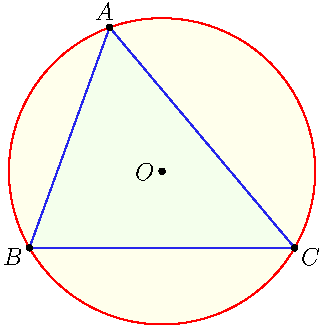
\includegraphics[width=5.5cm]{figures/demo.pdf}
  \caption{最小 TSQX 示例渲染结果（\texttt{figures/demo.txt}）}
  \label{fig:demo}
\end{figure}

TSQX 文件由逐行排列的四类语句构成：点声明、绘制语句、快捷宏以及注释/原生注入。没有行尾分号，也不需要手写 \code{pair} 类型声明与 \code{dot(...)} 标注代码。

\section{点声明、点修饰符与标签方向}

点声明的完整语法格式为
\[
  \texttt{点名}\; [\texttt{标签方向}]\; [\texttt{修饰符}]\texttt{=}\; \texttt{表达式}.
\]

\subsection{点修饰符（控制黑点与字母显隐）}

\begin{table}[htbp]
  \centering
  \caption{点声明修饰符对照表（常规模式与 \texttt{-b} 软标注模式）}
  \label{tab:point-modifiers}
  \small
  \begin{tabular}{@{}lcccc@{}}
    \toprule
    修饰符写法 & 常规模式画点 & 常规模式贴字 & \code{-b} 模式画点 & \code{-b} 模式贴字 \\
    \midrule
    \code{=}（默认） & 是 & 是 & 否 & 是 \\
    \code{dl=} & 是 & 是 & 是 & 是 \\
    \code{:=} & 否 & 否 & 否 & 否 \\
    \code{.=} 或 \code{d=} & 是 & 否 & 是 & 否 \\
    \code{;=} 或 \code{l=} & 否 & 是 & 是 & 是 \\
    \bottomrule
  \end{tabular}
\end{table}

实际画图中，建议将仅用于过渡计算的辅助点写作 \code{:=}，将垂足、中点等不希望压黑点的点写作 \code{;=}。

\subsection{标签方向（4 种完整写法）}

点名之后、等号之前可紧跟一个方向词，控制字母相对点位的偏移方向：

\begin{table}[htbp]
  \centering
  \caption{TSQX 标签方向语法全集}
  \label{tab:label-dirs}
  \small
  \begin{tabularx}{\linewidth}{@{}>{\ttfamily}p{0.20\linewidth}>{\ttfamily}p{0.28\linewidth}X@{}}
    \toprule
    TSQX 写法 & 编译后的 Asymptote 参数 & 说明 \\
    \midrule
    （省略） & dir(P) & 沿原点至 \(P\) 的射线外推；对单位圆上的点效果良好，三角形内部点建议手动指定 \\
    N, NE, SW, E & plain.N, plain.NE & 罗盘方位简写，匹配 \code{N?S?E?W?} \\
    45, 270 & dir(45), dir(270) & 极角（单位为度），精细避让线段时最常用 \\
    2S3E, 1N2W & 2*plain.S+3*plain.E & 整数倍方位线性组合，拉大标签间距 \\
    1.5R30 & 1.5*dir(30) & 极坐标倍径偏移：沿 \(30^\circ\) 方向外推 \(1.5\) 倍距离 \\
    \bottomrule
  \end{tabularx}
\end{table}

\subsection{特殊点名自动转义}

Asymptote 标识符不允许包含撇号或星号，TSQX 会自动转换：
\begin{itemize}
  \item \code{P'} 转为变量 \code{P\_prime}，标签自动渲染为 \(P'\)；
  \item \code{P\&} 转为变量 \code{P\_asterisk}，标签自动渲染为 \(P^{\ast}\)；
  \item \code{A\_1}、\code{M\_a}、\code{I\_A} 保持原名，标签直接按数学模式渲染为 \(A_1\)、\(M_a\)、\(I_A\)。
\end{itemize}

\section{表达式语法、路径连接与变换}

TSQX 表达式默认采用类 Lisp 前缀写法，同时兼容逗号分隔的函数调用：
\begin{lstlisting}[language={}]
# 前缀写法与括号写法等价
D = foot A B C
D = foot(A, B, C)
# 嵌套表达式用括号分组
K = extension A (foot A B C) B (midpoint A--C)
# 变换复合（从右向左作用，编译为乘积 *）
F' N = (rotate -30 E)(extension A (foot A B C) C E)
Q = (shift (0, 1))(reflect A B)(C)
\end{lstlisting}

路径连接符支持三种 Asymptote 原生记号：
\begin{itemize}
  \item \code{A--B--C--cycle}：折线与闭合多边形；
  \item \code{A..B..C..cycle}：光滑样条曲线；
  \item \code{\textasciicircum\textasciicircum}：子路径连接符（注意用于组合简单路径时需避免括号嵌套陷阱，见第~\ref{chap:pitfalls} 章）。
\end{itemize}

\section{绘制语句与快捷宏}

绘制语句使用斜杠 \code{/} 分隔几何对象、填充笔与描边笔：
\begin{lstlisting}[language={}]
A--B--C--cycle                         # 仅默认描边：draw(A--B--C--cycle);
A--D / dashed blue                     # 仅指定描边：draw(A--D, dashed+blue);
A--B--C--cycle / 0.12 lightcyan / blue # 填充+描边：filldraw(..., opacity(0.12)+lightcyan, blue);
circumcircle A B C / 0.15 lightgray /  # 填充+默认描边：filldraw(..., opacity(0.15)+lightgray, defaultpen);
\end{lstlisting}

\begin{warnbox}
\textbf{切勿省略斜杠 \code{/}}。早期示例曾误写为 \code{B--F dashed blue}，实际会被 \code{tsqx} 翻译成非法的 \code{draw(B--F, dashed, blue);} 并导致 Asymptote 报错。只要指定了任意颜色、线型或语义笔名，必须写 \code{/}，例如 \code{B--F / dashed blue} 或 \code{B--F / aux}。
\end{warnbox}

快捷宏以波浪号 \code{\~{}} 开头，上游解析器共内置两条：
\begin{itemize}
  \item \code{\~{}triangle A B C}：等价于依次声明 \code{A = dir 110}、\code{B = dir 210}、\code{C = dir 330}。它\textbf{只生成三个顶点，不会设置图形尺寸}。
  \item \code{\~{}regular A B C D E}：在单位圆上从 \(90^\circ\) 起逆时针等分生成正 \(n\) 边形顶点。
\end{itemize}

\section{命令行参数与原生逃生舱}

表~\ref{tab:cli-flags} 汇总了 \code{tsqx} 命令的全部常用选项。

\begin{table}[htbp]
  \centering
  \caption{\texttt{tsqx} 命令行参数说明}
  \label{tab:cli-flags}
  \small
  \begin{tabularx}{\linewidth}{@{}>{\ttfamily}p{0.22\linewidth}X@{}}
    \toprule
    选项 & 作用与使用建议 \\
    \midrule
    -p, --pre & 附加独立编译所需的 Asymptote 前导代码（含 \code{import geometry;}、\code{foot}、\code{CP} 等与 \code{size(...)}）。独立出图必加。 \\
    -s, --size <长度> & 覆盖前导中的默认尺寸 \code{8cm}，例如 \code{-s 7.5cm}。 \\
    -b, --soft-label & 默认 \code{=} 只贴字母不画点，\code{;=} 改为既画点又贴字。 \\
    -t, --terse & 省略输出 \code{.asy} 末尾附带的原始 TSQX 注释块。 \\
    filename & 从指定文件读入；省略时从标准输入读取。 \\
    \bottomrule
  \end{tabularx}
\end{table}

行首以 \code{!} 开头的语句原样透传给 Asymptote，行内 \code{\#} 之后为注释。借助 \code{!} 可以声明复用的 \code{!path}、编写辅助函数、执行二分数值求解，或插入第~\ref{chap:workflow} 章的几何不变量断言。

% ============================================================================
\chapter{内置几何函数与官方 Wiki 差异真相}
\label{chap:functions}
% ============================================================================

查阅上游 \code{vEnhance/tsqx} 官方 Wiki 时，初学者最常遇到的困惑是：照着 Wiki 抄了 \code{anglemark}、\code{rightanglemark} 或 \code{bisectorpoint}，编译却直接报 \code{no matching variable}。原因在于官方 Wiki 仍沿用原作者本机额外安装的 \code{olympiad.asy} 与 \code{cse5.asy}，而标准 \code{pip install tsqx} 在 \code{-p} 导言里实际加载的是 Asymptote 标准库 \code{import geometry;} 加上 8 个替代函数。

\section{标准 \texttt{tsqx -p} 直接可用的全部几何函数}

表~\ref{tab:verified-builtins} 列出所有经过 PyPI \code{tsqx} 与 Asymptote 2.87 逐条编译通过的函数。

\begin{table}[htbp]
  \centering
  \caption{标准 \texttt{tsqx -p} 环境实测直接可用的函数清单}
  \label{tab:verified-builtins}
  \small
  \begin{tabularx}{\linewidth}{@{}p{0.12\linewidth}>{\ttfamily}p{0.31\linewidth}X@{}}
    \toprule
    分类 & 函数写法 & 几何含义与参数说明 \\
    \midrule
    顶点与心 & dir 110 & 单位圆上 \(110^\circ\) 处的点 \\
             & incenter A B C & \(\triangle ABC\) 的内心 \\
             & circumcenter A B C & \(\triangle ABC\) 的外心 \\
             & orthocenter A B C & \(\triangle ABC\) 的垂心 \\
             & centroid A B C & \(\triangle ABC\) 的重心 \\
             & excenter A B C & 对应顶点 \(A\) 的旁心（\code{geometry} 自带，Wiki 未列） \\
    点构造   & midpoint A--B & 线段（或路径）\(AB\) 的中点 \\
             & foot P A B & 点 \(P\) 到直线 \(AB\) 的垂足（\textbf{先写点，再写直线两点}） \\
             & extension A B C D & 直线 \(AB\) 与直线 \(CD\) 的交点 \\
             & IP p q / OP p q & 路径 \(p, q\) 的第 0 / 第 1 个交点（顺序不保证特定分支） \\
    几何变换 & (rotate a O)(P) & 将 \(P\) 绕 \(O\) 逆时针旋转 \(a^\circ\) \\
             & (reflect A B)(P) & 将 \(P\) 关于直线 \(AB\) 对称反射 \\
             & (scale k O)(P) & 以 \(O\) 为中心将 \(P\) 缩放 \(k\) 倍 \\
             & (shift v)(P) & 将 \(P\) 按向量 \(v\) 平移 \\
    圆与直线 & circumcircle A B C & \(\triangle ABC\) 的外接圆 \\
             & incircle A B C & \(\triangle ABC\) 的内切圆 \\
             & CP O A & 以 \(O\) 为圆心、过点 \(A\) 的圆 \\
             & CR O r & 以 \(O\) 为圆心、半径为 \(r\) 的圆 \\
             & unitcircle & 单位圆 \\
             & Line A B & 过 \(A, B\) 两端各外延 \(0.6\) 倍长度的线段 \\
    前缀算术 & plus / minus / mult / divide & 对应四则运算，可规避中缀空格歧义 \\
    \bottomrule
  \end{tabularx}
\end{table}

\section{官方 Wiki 列出但默认缺失的 8 个函数及 \texttt{ldgeo.asy} 补完}

为解决“照着 Wiki 写却编不过”以及“每道题都重复手写垂线/切线/另一交点 helper”的痛点，本仓库在 \code{templates/tsqx/ldgeo.asy} 中集中补齐了这些高频竞赛函数，并全部经过实测。表~\ref{tab:wiki-diff} 给出了完整对照。

\begin{table}[htbp]
  \centering
  \caption{官方 Wiki 与标准 \texttt{tsqx -p} 的 8 处差异及 \texttt{ldgeo.asy} 替代写法}
  \label{tab:wiki-diff}
  \small
  \begin{tabularx}{\linewidth}{@{}>{\ttfamily}p{0.25\linewidth}p{0.27\linewidth}>{\ttfamily}X@{}}
    \toprule
    Wiki 写法 & 标准 \texttt{tsqx -p} 实测结果 & \texttt{ldgeo.asy} 一行替代写法 \\
    \midrule
    rightanglemark A B C & 报错：未定义变量 & rightanglemark A B C / mark \\
    anglemark A B C & 报错：未定义变量 & anglemark A B C / mark \\
    pathticks (A--B) 2 & 报错：未定义变量 & pathtick A B 2 / mark \\
    bisectorpoint A B C & 报错：未定义变量 & bisectorPt A B C（外分用 extBisectorPt） \\
    tangent P c 1 & 报错：无匹配重载 & tangentPt P O A 1 或 tangentPtR P O r 1 \\
    IP p q n（三参数） & 报错：仅支持两参数 & other c l X 或 otherPt c A B \\
    intersect p q & 返回 \code{real[]} 而非 \code{pair} & 直线用 extension；圆线用 otherPt \\
    arc A B a1 a2 & 报错：第二参数应为半径 & !draw(arc(O, abs(A-O), a1, a2), circ); \\
    \bottomrule
  \end{tabularx}
\end{table}

此外，\code{ldgeo.asy} 还补充了竞赛中最常用的四个构造器：
\begin{itemize}
  \item \code{perpPt P A B}：过 \(P\) 且垂直于 \(AB\) 的直线上一点，配合 \code{extension} 可一行构造任意垂线交点，例如 \code{T = extension B (perpPt B O B) C (perpPt C O C)}。
  \item \code{paraPt P A B}：过 \(P\) 且平行于 \(AB\) 的直线上一点，配合 \code{extension} 一行构造平行线截点。
  \item \code{otherPt c A B}：自动按曲线 \(c\) 的包围盒延展直线 \(AB\)，返回直线 \(AB\) 与圆 \(c\) 除已知点 \(A\) 之外的另一交点。
  \item \code{radicalAxis O1 r1 O2 r2 halfLen}：直接生成两圆的根轴线段路径。
\end{itemize}

% ============================================================================
\chapter{解析器词法边界与避坑指南}
\label{chap:pitfalls}
% ============================================================================

TSQX 解析器全长不足 500 行，采用轻量字符串分词而非完整语法树。理解下面五类边界行为，可以省去绝大多数无谓排错。

\section{陷阱一：绘制样式漏写斜杠 \texttt{/}}

如第 3 章所述，\code{A--B dashed blue} 会被翻译为 \code{draw(A--B, dashed, blue);}，Asymptote 会将第二个参数当成字符串标签从而编译失败。任何带样式的绘制语句都必须写为 \code{A--B / dashed blue}。

\section{陷阱二：\texttt{/} 后不可书写带括号的笔刷函数}

在 TSQX 词法阶段，\code{tokenize()} 先于 \code{parse\_draw()} 运行，会将 \code{(} 与 \code{)} 拆成独立词素，随后 \code{parse\_draw()} 用 \code{+} 将所有词素拼接起来。因此：
\begin{lstlisting}[language={}]
# 以下三种写法全部会在 Asymptote 中报语法错误：
A--B / gray(0.5)            # 翻译为 draw(A--B, gray(+0.5+));
A--B / linewidth(1.5) red   # 翻译为 draw(A--B, linewidth(+1.5+)+red);
A--B / rgb("1B4F9C")        # 翻译为 draw(A--B, rgb(+"1B4F9C"+));
\end{lstlisting}

\textbf{正解}：将自定义颜色、线宽与虚线模式预先绑定为无括号的 Asymptote \code{pen} 变量名（即第~\ref{chap:themes} 章的语义笔令牌 \code{given}、\code{aux}、\code{key} 等），在 TSQX 中只需写 \code{A--B / aux}。个别临时特殊线型可用 \code{!draw(A--B, linewidth(1.5)+red);}。

\section{陷阱三：中缀算术空格与括号嵌套}

\code{tokenize()} 会尝试删除 \code{+ - *} 两侧的空格，但对含减号或多重括号的表达式并不总是安全：
\begin{itemize}
  \item \code{P = 2*A - B}（减号左侧带空格）会被错误翻译为 \code{pair P = 2*A(-B);}。应紧贴写作 \code{P = 2*A-B}，或使用前缀算术 \code{P = minus (2*A) B}。
  \item 复杂表达式如 \code{P = (B + 0.5*(lo+hi)*(C-B))} 容易触发括号分词错位。涉及多步代数计算时，先在 \code{!pair pP = ...;} 中算好，再写 \code{P 270 = pP}。
\end{itemize}

\section{陷阱四：两个括号表达式直接用 \texttt{--} 相连}

上游解析器测试用例中已暴露一个历史行为：\code{(foot A B C)--(foot B C A)} 会被翻译成非法的 \code{foot(A, B, C)*-(-)*foot(B, C, A)}。写法规范是先命名端点再连线：
\begin{lstlisting}[language={}]
D := foot A B C
E := foot B C A
D--E / aux
\end{lstlisting}

\section{陷阱五：把 \texttt{OP} 当作“除已知顶点之外的另一交点”}

\begin{warnbox}
\textbf{高频几何错误}：\code{IP p q} 与 \code{OP p q} 只是取 \code{intersectionpoints(p, q)[0]} 和 \code{[1]}。两条路径的交点编号取决于 Asymptote 内部路径起点与方向，\textbf{并不保证 \code{OP} 一定是你想要的那一支}。一旦稍微调整顶点角度，\code{OP} 可能突然跳回已知顶点 \(A\)，导致整张图退化。
\end{warnbox}

此外，默认 \code{Line A B} 仅在 \(A, B\) 两端各延展 \(0.6\) 倍线段长，遇到较远的圆交点时常因线段不够长而报数组越界。在启用 \code{ldgeo.asy} 后，统一使用 \code{otherPt w A B}（自动延展并严格选取离 \(A\) 更远的交点）即可根治此类错误。

% ============================================================================
\chapter{排版美学与 CSS 式语义化配色系统}
\label{chap:themes}
% ============================================================================

\section{竞赛几何图的五层视觉信息分级}

许多自制几何图显得凌乱，并非因为构造复杂，而是把颜色当成了随意装饰——同一张图混用七八种高饱和纯色、线宽完全一致，导致读者的视线无法在第一时间分辨题设骨架与待证结论。按视觉传达原则，一张竞赛几何图只需划分为五个层次：
\begin{enumerate}
  \item \textbf{基底填色（\code{fill1} / \code{fill2} / \code{fillkey}）}：极低不透明度（\(0.08\)--\(0.12\)），用于衬托参考三角形或目标圆域，绝不压过线条。
  \item \textbf{已知骨架（\code{given}）}：深炭黑、标准线宽（\(0.75\,\mathrm{pt}\)），承接主三角形与已知多边形。
  \item \textbf{构造圆系（\code{circ} / \code{circ2}）}：中等明度主色（如深蓝、松柏绿），略细线宽（\(0.70\,\mathrm{pt}\)），避免大圆压迫内部细节。
  \item \textbf{辅助线与几何标记（\code{aux} / \code{aux2} / \code{mark}）}：中性灰虚线/点线（\(0.50\)--\(0.55\,\mathrm{pt}\)），视觉退居背景，不干扰主线。
  \item \textbf{核心结论与焦点（\code{key} / \code{accent}）}：高对比强调色并适度加粗（\(0.95\)--\(1.05\,\mathrm{pt}\)），整张图严格控制在两类焦点以内。
\end{enumerate}

\section{零样板源码 + 编译期注入机制}

借助 Asymptote 的 \code{-autoimport ldgeo -u <theme>} 启动选项，可以实现类似 HTML 与 CSS 分离的架构：
\begin{itemize}
  \item \textbf{\code{.tsqx} 源码保持零样板}：只需写语义令牌名（如 \code{A--D / aux}、\code{O--H / key}），无需写 \code{!import}，也完全兼容原版 \code{tsqx} 命令行工具。
  \item \textbf{改一个参数全篇换肤}：同一套 \code{.tsqx} 源码在讲义里用 \code{colormath} 或 \code{classic}，印成校内黑白试卷时只需改为 \code{--theme print}，放进 16:9 投影课件时改为 \code{--theme slides}。
  \item \textbf{对外分享独立可编}：使用 \code{scripts/build\_tsqx.py --standalone} 或 VS Code 命令面板导出时，工具会自动把 \code{ldgeo.asy} 与当前主题内联进 \code{.asy} 文件头，收件人无需配置外部库即可直接运行 \code{asy}。
\end{itemize}

表~\ref{tab:semantic-tokens} 列出了 \code{templates/tsqx/ldgeo.asy} 定义的全部 11 个语义笔令牌。

\begin{table}[htbp]
  \centering
  \caption{\texttt{ldgeo.asy} 语义笔令牌全表}
  \label{tab:semantic-tokens}
  \small
  \begin{tabularx}{\linewidth}{@{}>{\ttfamily}p{0.15\linewidth}p{0.23\linewidth}X@{}}
    \toprule
    令牌名 & 视觉层级 & 适用几何对象 \\
    \midrule
    given & 已知骨架（实线） & 主三角形、已知四边形边 \\
    aux & 主辅助线（虚线） & 高线、中线、角平分线、延长线 \\
    aux2 & 次辅助线（点线） & 半径辅助线、垂足连线、中位线 \\
    key & 第一核心结论（加粗） & 欧拉线、根轴、极线、待证共线 \\
    accent & 第二重点强调 & 切线、垂足三角形、第二条核心路径 \\
    circ & 主圆 & 外接圆、题设主圆 \\
    circ2 & 次圆 & 内切圆、九点圆、第二个相交圆 \\
    mark & 几何标记（细实线） & 直角标 \code{rightanglemark}、角弧 \code{anglemark}、刻度 \code{pathtick} \\
    fill1 & 主基底淡填色 & 参考三角形或主圆底色 \\
    fill2 & 次区域淡填色 & 垂足三角形、内切圆或第二圆底色 \\
    fillkey & 重点区域淡填色 & 待重点关注的局部区域 \\
    \bottomrule
  \end{tabularx}
\end{table}

\section{五套预设主题实景对比}

图~\ref{fig:theme-gallery} 展示了\textbf{完全相同的同一份 \code{figures/theme\_demo.tsqx} 源码}，仅切换 \code{--theme} 参数后由 Asymptote 实时渲染出的五种视觉风格。其中 \code{print} 主题专门使用纯灰阶与四种线型/线宽组合，且以实色淡灰代替 PDF 半透明通道，避免部分黑白激光打印机将透明图层印成灰黑块；\code{colormath} 直接复用本仓库 \code{ColorMath.cls} 色板；\code{slides} 对齐 \code{exercise-slides.sty} 并将字号与线宽放大约 \(40\%\) 以适应教室投屏。

\begin{figure}[htbp]
  \centering
  \begin{tabular}{@{}ccc@{}}
    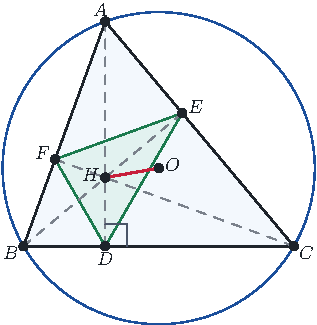
\includegraphics[width=0.31\linewidth]{figures/theme_demo_classic.pdf} &
    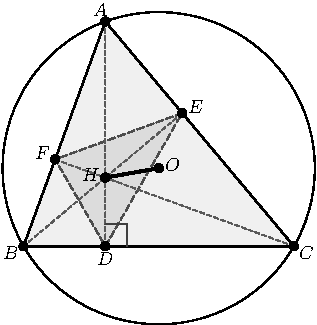
\includegraphics[width=0.31\linewidth]{figures/theme_demo_print.pdf} &
    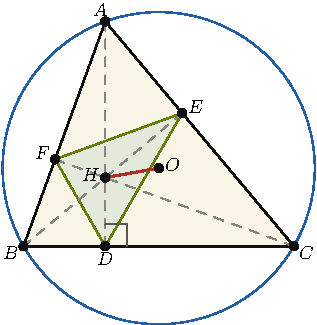
\includegraphics[width=0.31\linewidth]{figures/theme_demo_flexoki.pdf} \\
    \small\texttt{classic}（默认讲义） & \small\texttt{print}（黑白试卷） & \small\texttt{flexoki}（护眼纸感） \\[1.0em]
  \end{tabular}
  \begin{tabular}{@{}cc@{}}
    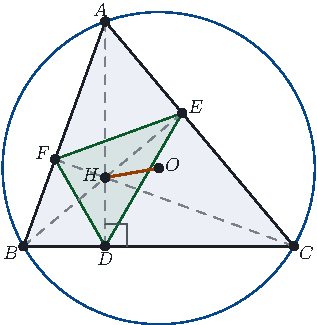
\includegraphics[width=0.31\linewidth]{figures/theme_demo_colormath.pdf} &
    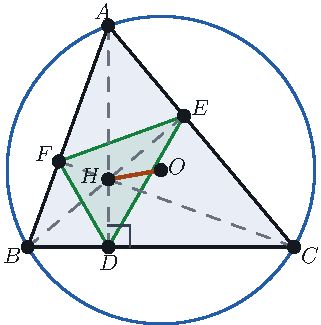
\includegraphics[width=0.31\linewidth]{figures/theme_demo_slides.pdf} \\
    \small\texttt{colormath}（ColorMath 色板） & \small\texttt{slides}（16:9 投影加粗）
  \end{tabular}
  \caption{同一份 \texttt{theme\_demo.tsqx} 源码在五套 \texttt{ldgeo} 预设主题下的渲染对比}
  \label{fig:theme-gallery}
\end{figure}

\section{物理画幅与 \LaTeX{} 字号 1:1 对齐原则}

一个经常被忽视的排版问题是：TSQX 内部以 \code{size(W)} 决定画布物理宽度，并按字号 \code{9.5pt}（由 \code{defaultpen} 设定）排版标签字母 \(A, B, C\)；如果在 \LaTeX{} 中再用 \code{\textbackslash includegraphics[width=W']} 强行缩放，则图中实际字号会变成
\[
  s_{\text{actual}} = 9.5\,\mathrm{pt} \times \frac{W'}{W}.
\]
例如以 \code{size(13cm)} 出图却在半栏缩成 \(5.5\,\mathrm{cm}\)，字母会缩小到约 \(4\,\mathrm{pt}\)，印刷后几乎不可辨认；反之过度放大则会使线条与标签显得笨拙。

推荐在整个讲义仓库统一采用三档物理画幅，并在 \code{.tex} 中按 \(1:1\) 物理宽度嵌入：
\begin{itemize}
  \item \code{--scale compact}（\(5.5\,\mathrm{cm}\)）：双栏图、并排对照图、小题配图；
  \item \code{--scale standard}（\(7.5\,\mathrm{cm}\)）：正文单栏标准例题配图；
  \item \code{--scale wide}（\(11.5\,\mathrm{cm}\)）：多圆、根轴或分步综合大图。
\end{itemize}

在讲义项目中，只需在 \code{project.yaml} 写一行 \code{tsqx\_theme: colormath}（或在图形目录放置 \code{.tsqxrc.json}），运行 \code{python3 scripts/build\_tsqx.py <项目目录>} 即可自动按项目配置批量构建全部插图。

% ============================================================================
\chapter{竞赛几何经典构型图鉴}
\label{chap:gallery}
% ============================================================================

本章给出 8 个由浅入深的竞赛平面几何典例。全部源码均位于 \code{figures/} 目录，均使用语义笔令牌编写，并附带几何不变量断言，经过 \code{scripts/build\_tsqx.py --theme classic --scale standard --standalone} 实测编出。

\section{例 1：内心、内切圆与切点垂足}

构型要点：使用 \code{\~{}triangle} 快速铺设一般锐角三角形，利用 \code{incenter} 与 \code{foot} 得到内心 \(I\) 及三切点 \(D, E, F\)，并用 \code{!check\_perp} 与 \code{!check\_equal\_dist} 验算内切圆半径相等。

\lstinputlisting[language={}]{figures/fig1.tsqx}

\begin{figure}[htbp]
  \centering
  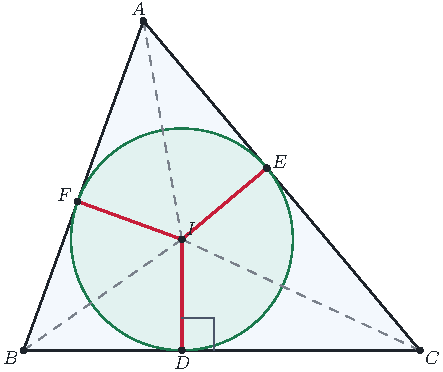
\includegraphics[width=7.5cm]{figures/fig1.pdf}
  \caption{例 1：内心、内切圆与切点垂足（\texttt{figures/fig1.tsqx}）}
  \label{fig:ex1}
\end{figure}

\section{例 2：垂心、垂足三角形与欧拉线}

构型要点：同时构造外心 \(O\)、重心 \(G\)、垂心 \(H\) 与垂足三角形 \(DEF\)，通过 \code{!check\_collinear(O, G, H, ...)} 自动验证欧拉线共线。使用 \code{accent} 区分垂足三角形轮廓，\code{key} 突出欧拉线 \(OH\)。

\lstinputlisting[language={}]{figures/fig2.tsqx}

\begin{figure}[htbp]
  \centering
  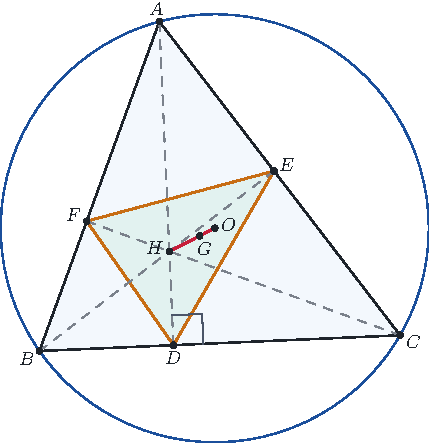
\includegraphics[width=7.5cm]{figures/fig2.pdf}
  \caption{例 2：垂心、垂足三角形与欧拉线（\texttt{figures/fig2.tsqx}）}
  \label{fig:ex2}
\end{figure}

\section{例 3：鸡爪定理（Fact 5）}

构型要点：以 \(L = \mathrm{dir}\,270\) 作为弧 \(BC\) 中点，直接利用中心对称表达式 \code{(2*L-I)} 得到 \(A\)-旁心 \(I_A\)，再以 \code{CP L I} 绘出以 \(L\) 为圆心、同时经过 \(B, I, C, I_A\) 的特征圆。

\lstinputlisting[language={}]{figures/fig3.tsqx}

\begin{figure}[htbp]
  \centering
  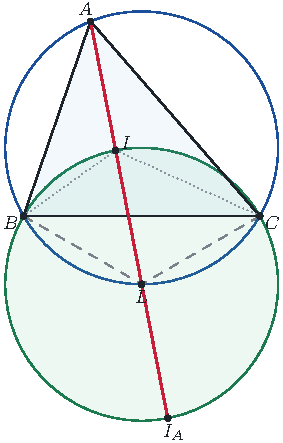
\includegraphics[width=7.5cm]{figures/fig3.pdf}
  \caption{例 3：鸡爪定理构型（\texttt{figures/fig3.tsqx}）}
  \label{fig:ex3}
\end{figure}

\section{例 4：九点圆}

构型要点：依次构造三边中点 \(M_a, M_b, M_c\)、三高垂足 \(D, E, F\) 与欧拉中点 \(K_a, K_b, K_c\)，并用多条 \code{!check\_cyclic} 断言自动核验其余六点确实落在 \(\triangle M_a M_b M_c\) 的外接圆上。通过将顶点 \(A\) 调整至 \code{dir 118}，有效拉开垂足 \(E, F\) 与中点 \(M_b, M_c\) 的间距，避免标签拥挤。

\lstinputlisting[language={}]{figures/fig4_ninepoint.tsqx}

\begin{figure}[htbp]
  \centering
  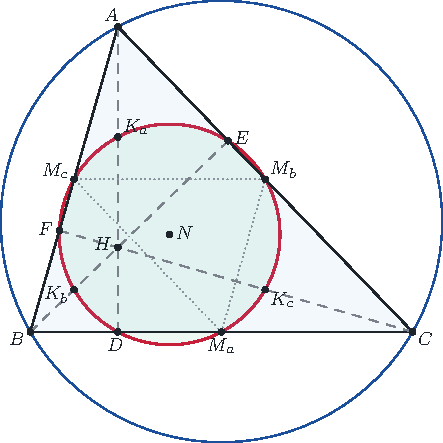
\includegraphics[width=7.5cm]{figures/fig4_ninepoint.pdf}
  \caption{例 4：九点圆（\texttt{figures/fig4\_ninepoint.tsqx}）}
  \label{fig:ex4}
\end{figure}

\section{例 5：三圆两两根轴与根心}

构型要点：使用 \code{ldgeo.asy} 提供的 \code{radicalAxis} 构造三圆的两两根轴线段，取其中两条交点作为根心 \(R\)，并用 \code{!check\_collinear} 验证 \(R\) 严格落在第三条根轴上。

\lstinputlisting[language={}]{figures/fig5_radical_axis.tsqx}

\begin{figure}[htbp]
  \centering
  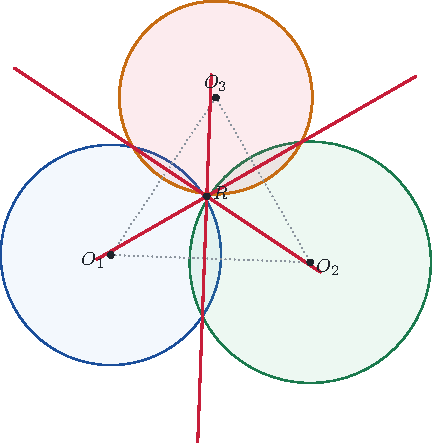
\includegraphics[width=7.5cm]{figures/fig5_radical_axis.pdf}
  \caption{例 5：三圆根轴与根心（\texttt{figures/fig5\_radical\_axis.tsqx}）}
  \label{fig:ex5}
\end{figure}

\section{例 6：外接圆切线、陪位中线与 \texttt{otherPt} 避坑}

构型要点：借助 \code{perpPt B O B} 与 \code{extension} 求 \(B, C\) 处切线交点 \(T\)；再通过 \code{otherPt w A T} 与 \code{otherPt w A M} 安全获取陪位中线、中线与外接圆的另一交点 \(K, D\)，彻底规避 \code{OP} 交点顺序不稳定的隐患，并配合 \code{pathtick} 与 \code{rightanglemark} 标注等长与相切。

\lstinputlisting[language={}]{figures/fig6_tangents_other.tsqx}

\begin{figure}[htbp]
  \centering
  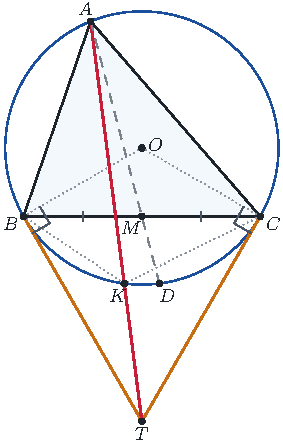
\includegraphics[width=7.5cm]{figures/fig6_tangents_other.pdf}
  \caption{例 6：切线、陪位中线与安全交点构造（\texttt{figures/fig6\_tangents\_other.tsqx}）}
  \label{fig:ex6}
\end{figure}

\section{例 7：圆外一点切线与极线（调和点列）}

构型要点：调用 \code{tangentPtR P O 1 1} 与 \code{tangentPtR P O 1 2} 从圆外点 \(P\) 向单位圆引两条切线得切点 \(A, B\)（按半径求切点用 \code{tangentPtR}，按圆上已知点求切点用 \code{tangentPt}，消除 Asymptote 整数重载歧义），再用 \code{otherPt} 作割线 \(PCD\) 与极线 \(AB\) 交于调和共轭点 \(Q\)。

\lstinputlisting[language={}]{figures/fig7_harmonic.tsqx}

\begin{figure}[htbp]
  \centering
  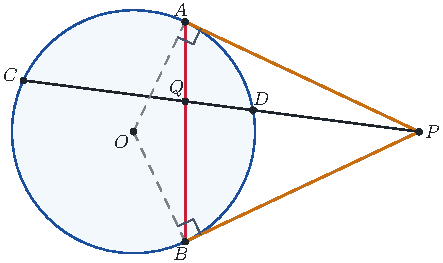
\includegraphics[width=7.5cm]{figures/fig7_harmonic.pdf}
  \caption{例 7：圆外切线与调和极线（\texttt{figures/fig7\_harmonic.tsqx}）}
  \label{fig:ex7}
\end{figure}

\section{例 8：隐式角度条件的数值二分求解与断言}

构型要点：部分联赛题包含难以尺规直接写出的隐式条件（如在线段 \(BC\) 上求点 \(P\) 使 \(\angle BAP = 2\angle ACB\)）。此时可在行首 \code{!} 块中编写 15 行二分求解器，再将结果赋给 TSQX 点变量，并附带严格断言。若初始三角形角度不满足解的存在性（例如 \(\angle BAC \le 2\angle ACB\)），断言会在编译阶段直接报错中止，防止生成貌似合理实则错误的配图。

\lstinputlisting[language={}]{figures/fig8_solver_assert.tsqx}

\begin{figure}[htbp]
  \centering
  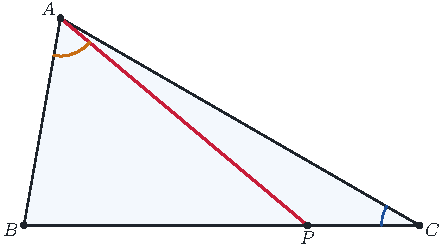
\includegraphics[width=7.5cm]{figures/fig8_solver_assert.pdf}
  \caption{例 8：隐式角度条件二分求解与断言验证（\texttt{figures/fig8\_solver\_assert.tsqx}）}
  \label{fig:ex8}
\end{figure}

% ============================================================================
\chapter{自然语言驱动配图：AI + Skill + 插件工作流}
\label{chap:workflow}
% ============================================================================

\section{四步闭环流程}

面对一道只有文字题干的竞赛平面几何题，最快且最可靠的生产流程由四个阶段组成：
\begin{enumerate}
  \item \textbf{自然语言交由 \code{tsqx-gen} Skill 解析}：AI 先拆解自由点、派生点、共线/垂直/相切/共圆约束，区分“题设真值”与“示意图猜测”，随后生成采用 \code{ldgeo} 语义笔令牌且内含 \code{!check\_*} 断言的 \code{.tsqx} 代码。
  \item \textbf{自动化编译与几何断言校验}：运行 \code{verify\_tsqx\_pipeline.py --pre --theme classic --check-png} 或在 VS Code 中按保存触发 \code{tsqx-compiler}。若构造违背题设约束，\code{assert} 会直接阻断输出；若交点跑飞导致画面纵横比超过 \(4:1\)，脚本会给出尺寸预警。
  \item \textbf{视觉目检与标签微调}：对照生成的 PNG 或 VS Code 持久 SVG 预览，仅调整少数点的标签方向角（如将 \code{M 270} 改为 \code{M 235}）或微调自由顶点角度（如把 \code{A = dir 110} 改为 \code{dir 118}）。
  \item \textbf{按载体批量换肤进讲义}：定稿后将 \code{.tsqx} 归档进项目 \code{figures/} 目录；讲义用 \code{--theme colormath}，黑白试卷用 \code{--theme print}，投影习题课用 \code{--theme slides}，一条命令完成全目录重编。
\end{enumerate}

\section{写给 AI 的高效几何提示词要点}

向挂载了 \code{tsqx-gen} Skill 的 AI 下达配图请求时，补充以下三点说明可明显提升首轮出图质量：
\begin{itemize}
  \item \textbf{明确图形用途}：写清“仅画题干原图（不剧透辅助线）”还是“画解法分步图（需突出根轴/共圆）”。
  \item \textbf{说明载体与尺度}：注明“单栏讲义标准图（\code{standard}, \code{classic}）”或“双栏黑白试卷图（\code{compact}, \code{print}）”。
  \item \textbf{标明需要锁定的视觉朝向}：例如“让底边 \(BC\) 水平，\(AB < AC\)，点 \(P\) 落在优弧 \(BC\) 上”。
\end{itemize}

\section{出图验收三道防线}

工具链编译通过仅代表语法合法，交付讲义前须逐项确认：
\begin{enumerate}
  \item \textbf{语法与编译通过}：\code{tsqx} 与 \code{asy} 返回码均为 \(0\)，生成非空 PDF。
  \item \textbf{几何不变量通过}：至少对题干中的 1--3 项关键垂直、共线、共圆、相切或等距条件通过 \code{!check\_*} 断言。
  \item \textbf{视觉可读性通过}：无点名重叠压线、无圆弧被意外截断、黑白打印主题下线条层级清晰可辨、物理宽度与 \LaTeX{} 嵌入宽度保持 \(1:1\)。
\end{enumerate}

% ============================================================================
\appendix
\chapter{单页速查表（Cheat Sheet）}
% ============================================================================

\begin{table}[H]
  \centering
  \footnotesize
  \renewcommand{\arraystretch}{1.04}
  \begin{tabularx}{\linewidth}{@{}>{\bfseries}p{0.16\linewidth}>{\ttfamily\raggedright\arraybackslash}p{0.39\linewidth}>{\raggedright\arraybackslash}X@{}}
    \toprule
    分类 & 典型写法 & 说明 \\
    \midrule
    点修饰符 & P = / P := / P .= / P ;= & 点+字 / 隐藏 / 仅点 / 仅字 \\
    标签方向 & P 45 / P NE / P 2S3E / P 1.5R30 & 极角 / 方位 / 线性偏移 / 极径偏移 \\
    特殊点名 & P' / P\& / A\_1 & 自动渲染为 \(P'\) / \(P^{\ast}\) / \(A_1\) \\
    快捷宏 & \~{}triangle A B C & 单位圆 \(110^\circ, 210^\circ, 330^\circ\) \\
           & \~{}regular A B C D E & 单位圆正 \(n\) 边形 \\
    标准构造 & foot P A B & \(P\) 到直线 \(AB\) 垂足 \\
             & midpoint A--B & 线段 \(AB\) 中点 \\
             & extension A B C D & 直线 \(AB, CD\) 交点 \\
             & incenter / circumcenter / orthocenter / centroid / excenter & 三角形五心 \\
             & circumcircle / incircle / CP / CR & 常见圆对象 \\
    \code{ldgeo} 补完 & otherPt w A B & 直线 \(AB\) 与圆 \(w\) 除 \(A\) 外另一交点 \\
                      & perpPt P A B / paraPt P A B & 过 \(P\) 垂线 / 平行线辅助点 \\
                      & bisectorPt / extBisectorPt A B C & 内 / 外角平分线辅助点 \\
                      & tangentPt P O A 1 / tangentPtR P O r 1 & 圆外点向圆引切线的切点 \\
                      & rightanglemark / anglemark / pathtick & 直角标 / 角弧 / 等长刻度 \\
                      & radicalAxis O1 r1 O2 r2 halfLen & 两圆根轴路径 \\
    几何断言 & !check\_perp(A,B,C,D,"...") & 验证 \(AB \perp CD\) \\
             & !check\_parallel / check\_collinear & 验证平行 / 共线 \\
             & !check\_cyclic / check\_on\_circle / check\_equal\_dist & 验证四点共圆 / 点在圆上 / 等距 \\
    语义令牌 & given / aux / aux2 / key / accent & 骨架 / 虚辅助 / 点辅助 / 主焦点 / 次焦点 \\
             & circ / circ2 / mark / fill1 / fill2 / fillkey & 主圆 / 次圆 / 标记 / 三档淡填色 \\
    常用命令 & python3 scripts/build\_tsqx.py DIR --theme print & 整目录按黑白试卷主题重编 \\
             & python3 scripts/build\_tsqx.py f.tsqx --standalone & 导出内联 \code{ldgeo} 的独立 \code{.asy} \\
    \bottomrule
  \end{tabularx}
\end{table}

\backmatter
\chapter*{参考资料}
\addcontentsline{toc}{chapter}{参考资料}
\small
\begin{enumerate}
  \item Evan Chen \& CJ Quines, TSQX 上游仓库与源码：
        \url{https://github.com/vEnhance/tsqx}
  \item TSQX 官方 Wiki 文档：
        \url{https://github.com/vEnhance/tsqx/wiki/Documentation}
  \item Evan Chen, Asymptote Guide：
        \url{https://web.evanchen.cc/asyguide.html}
  \item \code{tsqx-compiler} VS Code 扩展与源码：
        \url{https://github.com/YZDame/tsqx-compiler}
  \item \code{tsqx-gen} AI 几何作图技能（LD Stack）：
        \url{https://github.com/YZDame/ld-stack}
  \item 仓库配套文档：\code{docs/syntax-reference.md}、\code{docs/theme-guide.md}、\code{docs/troubleshooting.md}。
\end{enumerate}

\normalsize
\chapter*{后记}
\addcontentsline{toc}{chapter}{后记}
2025 年以来，开源推理模型与编程智能体的演进速度远超预期。进入 2026 年，围绕工具调用、技能协议与本地编译验证建立起来的代理工作流，让“用自然语言直接描述数学问题并产出精确矢量图”从设想走向了日常可用。

在这一背景下重新审视 TSQX，它的价值反而更加清晰：简洁的声明式语法天然适合作为自然语言与底层精确绘图引擎之间的中间层。相比让模型直接吐出上百行坐标代码，先由 AI 生成二十行语义清晰的 TSQX，再通过几何断言校验与统一配色主题批量渲染，既大幅降低了人工核对的负担，也让整套讲义、试卷与课件能够长期保持一致的视觉水准。

本手册初版完成于 2026 年 3 月；本次全面修订对照上游解析器源码逐条核实了函数边界与词法陷阱，补齐了 \code{ldgeo.asy} 语义化主题体系、8 组竞赛构型典例以及完整的 AI 辅助配图闭环。工具的意义始终在于减少重复劳动，把精力留给真正的数学思考。

\bigskip
\begin{flushright}
  LeyuDame\\
  2026 年 3 月初版，2026 年 11 月修订
\end{flushright}

\end{document}
